\documentclass{standalone}
\usepackage{tikz}
\begin{document}
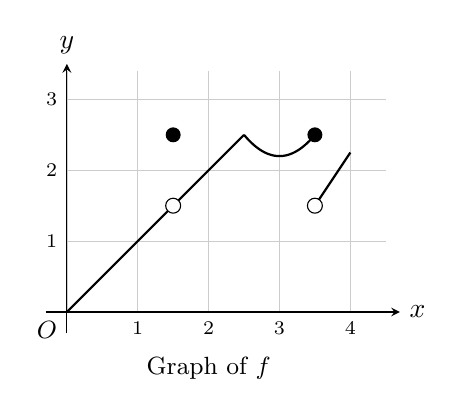
\begin{tikzpicture}[>=stealth, scale=0.9]
  % Gridlines (extended past the axes for a tic-tac-toe look)
  \draw[help lines, gray!40] (0,0) grid (4.5,3.4);

  % Axes
  \draw[->] (-0.3,0) -- (4.7,0) node[right] {$x$};
  \draw[->] (0,-0.3) -- (0,3.5) node[above] {$y$};

  \begin{scope}
    \clip (-0.3,-0.2) rectangle (4.6,3.4);
    % Linear segment from (0,0) to (2.5,2.5), slope 1
    \draw[thick] (0,0) -- (2.5,2.5);
    % Quadratic segment from x=2.5 to x=3.5, vertex (minimum) at x=3.0
    % y = 1.2*(x-3)^2 + 2.2, passing through (2.5,2.5) and (3.5,2.5)
    \draw[thick, domain=2.5:3.5, samples=50, smooth, variable=\x]
      plot (\x, {1.2*(\x-3)^2 + 2.2});
    % Linear segment from x=3.5 to x=4, slope 1.5, starting at (3.5,1.5)
    \draw[thick] (3.5,1.5) -- (4,2.25);
  \end{scope}

  % Hole at (1.5,1.5) on the first linear segment
  \draw[fill=white,draw=black] (1.5,1.5) circle (3pt);
  % Displaced filled point at (1.5,2.5)
  \fill[black] (1.5,2.5) circle (3pt);

  % End of quadratic: (3.5,2.5) is part of the function (filled)
  \fill[black] (3.5,2.5) circle (3pt);
  % Start of last linear segment: (3.5,1.5) is a hole
  \draw[fill=white,draw=black] (3.5,1.5) circle (3pt);

  % Axis tick labels
  \foreach \x in {1,2,3,4} {
    \node[below,font=\scriptsize] at (\x,0) {\x};
  }
  \foreach \y in {1,2,3} {
    \node[left,font=\scriptsize] at (0,\y) {\y};
  }
  \node[below left,font=\small] at (0,0) {$O$};

  % Title below
  \node[below,font=\small] at (2,-0.5) {Graph of $f$};
\end{tikzpicture}
\end{document}
